\documentclass[border=2pt]{standalone}
% Computer Modern, the font of the handouts (pdflatex)
\usepackage{amsmath}
\usepackage{tikz}
\usepackage{pgfplots}
\pgfplotsset{compat=1.18}
\usetikzlibrary{arrows.meta,calc}
\definecolor{cA}{HTML}{2A78D6}
\definecolor{cB}{HTML}{EB6834}
\definecolor{cC}{HTML}{1BAF7A}
\definecolor{cD}{HTML}{EDA100}
\definecolor{cE}{HTML}{E87BA4}
\definecolor{nodeblue}{HTML}{1565C0}
\definecolor{linkgray}{HTML}{546E7A}
\definecolor{lightgray}{HTML}{CFD8DC}
\definecolor{txt}{HTML}{263238}
\definecolor{band}{HTML}{EEEEEE}
\definecolor{uUnused}{HTML}{BDBDBD}
\definecolor{uLow}{HTML}{2E7D32}
\definecolor{uMid}{HTML}{F9A825}
\definecolor{uHigh}{HTML}{EF6C00}
\definecolor{uFull}{HTML}{C62828}
\definecolor{uOver}{HTML}{7B1FA2}
\tikzset{
  nd/.style={circle, fill=nodeblue, draw=white, line width=0.7pt, minimum size=#1, inner sep=0pt},
  nd/.default=3.2mm,
  nlab/.style={font=\footnotesize\bfseries, text=txt, inner sep=1pt},
  lbl/.style={font=\scriptsize, text=txt, fill=white, fill opacity=0.85, text opacity=1, inner sep=0.7pt},
  arr/.style={-{Stealth[length=1.9mm, width=1.5mm]}},
}
\pgfplotsset{
  lab/.style={
    scale only axis, axis lines*=left, grid=major, grid style={black!12},
    tick label style={font=\small}, label style={font=\normalsize},
    ylabel style={align=center},
    legend style={draw=none, fill=none, font=\small},
    legend cell align=left, tick align=outside, axis line style={black!60},
    every axis plot/.append style={line width=1.1pt},
  },
  % the series differ in color, marker and line style (readable in black and white);
  % the second series has hollow markers, visible where the two curves overlap
  s1/.style={cA, solid, mark=*, mark size=1.7pt},
  s2/.style={cB, densely dashed, mark=square*, mark size=1.6pt, mark options={solid, fill=white}},
  s3/.style={cC, dashdotted, mark=diamond*, mark size=2.1pt, mark options={solid}},
  s4/.style={cD, densely dotted, mark=triangle*, mark size=2.1pt, mark options={solid, fill=white}},
  s5/.style={cE, dashed, mark=triangle*, mark size=2.1pt, mark options={solid, rotate=180}},
  ebars/.style={error bars/.cd, y dir=both, y explicit,
    error bar style={solid, line width=0.9pt}, error mark options={solid, rotate=90, mark size=2.2pt}},
}
\begin{document}
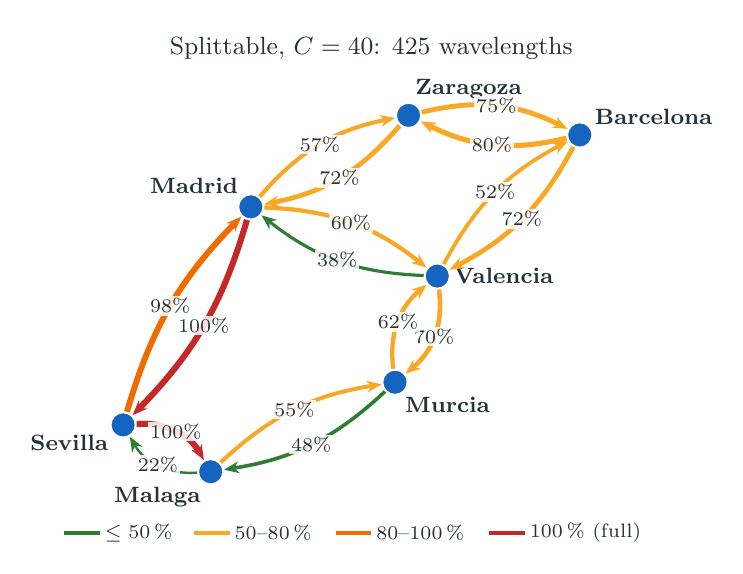
\begin{tikzpicture}
\node[nd=3.2mm, label={[nlab]135:Madrid}] (n0) at (1.622,3.364) {};
\node[nd=3.2mm, label={[nlab]30:Barcelona}] (n1) at (5.800,4.277) {};
\node[nd=3.2mm, label={[nlab]0:Valencia}] (n2) at (3.990,2.485) {};
\node[nd=3.2mm, label={[nlab]-150:Sevilla}] (n3) at (0.000,0.595) {};
\node[nd=3.2mm, label={[nlab]75:Zaragoza}] (n4) at (3.625,4.526) {};
\node[nd=3.2mm, label={[nlab]-120:Malaga}] (n5) at (1.112,0.000) {};
\node[nd=3.2mm, label={[nlab]-60:Murcia}] (n6) at (3.453,1.137) {};
\draw[arr, uMid, line width=1.48pt] (n0) to[bend left=19] node[lbl, midway] {57\%} (n4);
\draw[arr, uFull, line width=2.20pt] (n0) to[bend left=14] node[lbl, midway] {100\%} (n3);
\draw[arr, uMid, line width=1.52pt] (n0) to[bend left=18] node[lbl, midway] {60\%} (n2);
\draw[arr, uMid, line width=1.86pt] (n1) to[bend left=20] node[lbl, midway] {80\%} (n4);
\draw[arr, uMid, line width=1.73pt] (n1) to[bend left=17] node[lbl, midway] {72\%} (n2);
\draw[arr, uMid, line width=1.39pt] (n2) to[bend left=17] node[lbl, midway] {52\%} (n1);
\draw[arr, uMid, line width=1.69pt] (n2) to[bend left=29] node[lbl, midway] {70\%} (n6);
\draw[arr, uLow, line width=1.14pt] (n2) to[bend left=18] node[lbl, midway] {38\%} (n0);
\draw[arr, uFull, line width=2.20pt] (n3) to[bend left=32] node[lbl, midway] {100\%} (n5);
\draw[arr, uHigh, line width=2.16pt] (n3) to[bend left=14] node[lbl, midway] {98\%} (n0);
\draw[arr, uMid, line width=1.73pt] (n4) to[bend left=19] node[lbl, midway] {72\%} (n0);
\draw[arr, uMid, line width=1.77pt] (n4) to[bend left=20] node[lbl, midway] {75\%} (n1);
\draw[arr, uMid, line width=1.44pt] (n5) to[bend left=17] node[lbl, midway] {55\%} (n6);
\draw[arr, uLow, line width=0.88pt] (n5) to[bend left=32] node[lbl, midway] {22\%} (n3);
\draw[arr, uMid, line width=1.56pt] (n6) to[bend left=29] node[lbl, midway] {62\%} (n2);
\draw[arr, uLow, line width=1.31pt] (n6) to[bend left=17] node[lbl, midway] {48\%} (n5);
\node[font=\small, text=txt, anchor=south] at ($(current bounding box.north)+(0,1mm)$) {Splittable, $C = 40$: 425 wavelengths};
\coordinate (lg) at ($(current bounding box.south)+(0,-3mm)$);
\draw[uLow, line width=1.6pt] ($(lg)+(-39.0mm,0)$) -- ++(4.5mm,0) node[right, font=\scriptsize, text=txt, inner sep=1pt] {$\le 50\,\%$};
\draw[uMid, line width=1.6pt] ($(lg)+(-22.5mm,0)$) -- ++(4.5mm,0) node[right, font=\scriptsize, text=txt, inner sep=1pt] {50--80\,\%};
\draw[uHigh, line width=1.6pt] ($(lg)+(-4.5mm,0)$) -- ++(4.5mm,0) node[right, font=\scriptsize, text=txt, inner sep=1pt] {80--100\,\%};
\draw[uFull, line width=1.6pt] ($(lg)+(15.0mm,0)$) -- ++(4.5mm,0) node[right, font=\scriptsize, text=txt, inner sep=1pt] {100\,\% (full)};
\end{tikzpicture}
\hspace{4mm}
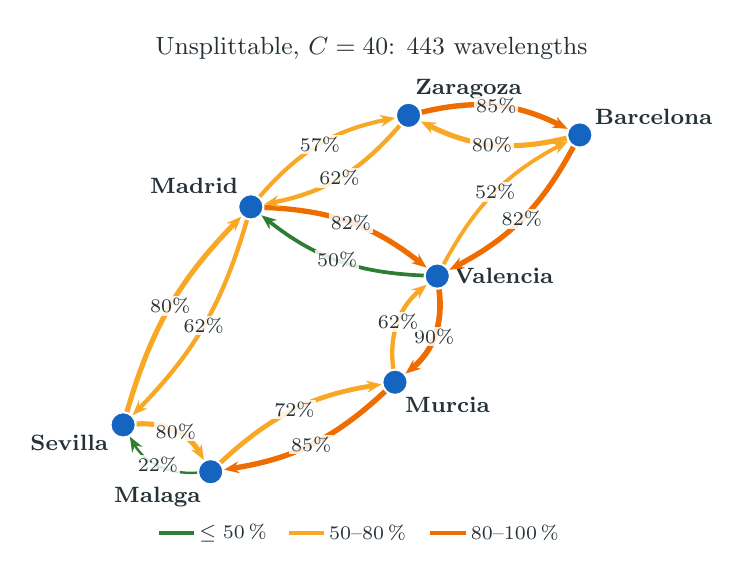
\begin{tikzpicture}
\node[nd=3.2mm, label={[nlab]135:Madrid}] (n0) at (1.622,3.364) {};
\node[nd=3.2mm, label={[nlab]30:Barcelona}] (n1) at (5.800,4.277) {};
\node[nd=3.2mm, label={[nlab]0:Valencia}] (n2) at (3.990,2.485) {};
\node[nd=3.2mm, label={[nlab]-150:Sevilla}] (n3) at (0.000,0.595) {};
\node[nd=3.2mm, label={[nlab]75:Zaragoza}] (n4) at (3.625,4.526) {};
\node[nd=3.2mm, label={[nlab]-120:Malaga}] (n5) at (1.112,0.000) {};
\node[nd=3.2mm, label={[nlab]-60:Murcia}] (n6) at (3.453,1.137) {};
\draw[arr, uMid, line width=1.48pt] (n0) to[bend left=19] node[lbl, midway] {57\%} (n4);
\draw[arr, uMid, line width=1.56pt] (n0) to[bend left=14] node[lbl, midway] {62\%} (n3);
\draw[arr, uHigh, line width=1.90pt] (n0) to[bend left=18] node[lbl, midway] {82\%} (n2);
\draw[arr, uMid, line width=1.86pt] (n1) to[bend left=20] node[lbl, midway] {80\%} (n4);
\draw[arr, uHigh, line width=1.90pt] (n1) to[bend left=17] node[lbl, midway] {82\%} (n2);
\draw[arr, uMid, line width=1.39pt] (n2) to[bend left=17] node[lbl, midway] {52\%} (n1);
\draw[arr, uHigh, line width=2.03pt] (n2) to[bend left=29] node[lbl, midway] {90\%} (n6);
\draw[arr, uLow, line width=1.35pt] (n2) to[bend left=18] node[lbl, midway] {50\%} (n0);
\draw[arr, uMid, line width=1.86pt] (n3) to[bend left=32] node[lbl, midway] {80\%} (n5);
\draw[arr, uMid, line width=1.86pt] (n3) to[bend left=14] node[lbl, midway] {80\%} (n0);
\draw[arr, uMid, line width=1.56pt] (n4) to[bend left=19] node[lbl, midway] {62\%} (n0);
\draw[arr, uHigh, line width=1.94pt] (n4) to[bend left=20] node[lbl, midway] {85\%} (n1);
\draw[arr, uMid, line width=1.73pt] (n5) to[bend left=17] node[lbl, midway] {72\%} (n6);
\draw[arr, uLow, line width=0.88pt] (n5) to[bend left=32] node[lbl, midway] {22\%} (n3);
\draw[arr, uMid, line width=1.56pt] (n6) to[bend left=29] node[lbl, midway] {62\%} (n2);
\draw[arr, uHigh, line width=1.94pt] (n6) to[bend left=17] node[lbl, midway] {85\%} (n5);
\node[font=\small, text=txt, anchor=south] at ($(current bounding box.north)+(0,1mm)$) {Unsplittable, $C = 40$: 443 wavelengths};
\coordinate (lg) at ($(current bounding box.south)+(0,-3mm)$);
\draw[uLow, line width=1.6pt] ($(lg)+(-27.0mm,0)$) -- ++(4.5mm,0) node[right, font=\scriptsize, text=txt, inner sep=1pt] {$\le 50\,\%$};
\draw[uMid, line width=1.6pt] ($(lg)+(-10.5mm,0)$) -- ++(4.5mm,0) node[right, font=\scriptsize, text=txt, inner sep=1pt] {50--80\,\%};
\draw[uHigh, line width=1.6pt] ($(lg)+(7.5mm,0)$) -- ++(4.5mm,0) node[right, font=\scriptsize, text=txt, inner sep=1pt] {80--100\,\%};
\end{tikzpicture}
\end{document}
